\documentclass{standalone}
\usepackage{pgfplots}
\usepackage{tikz}
\usepackage{amsmath}
\pgfplotsset{compat=1.16}

\begin{document}

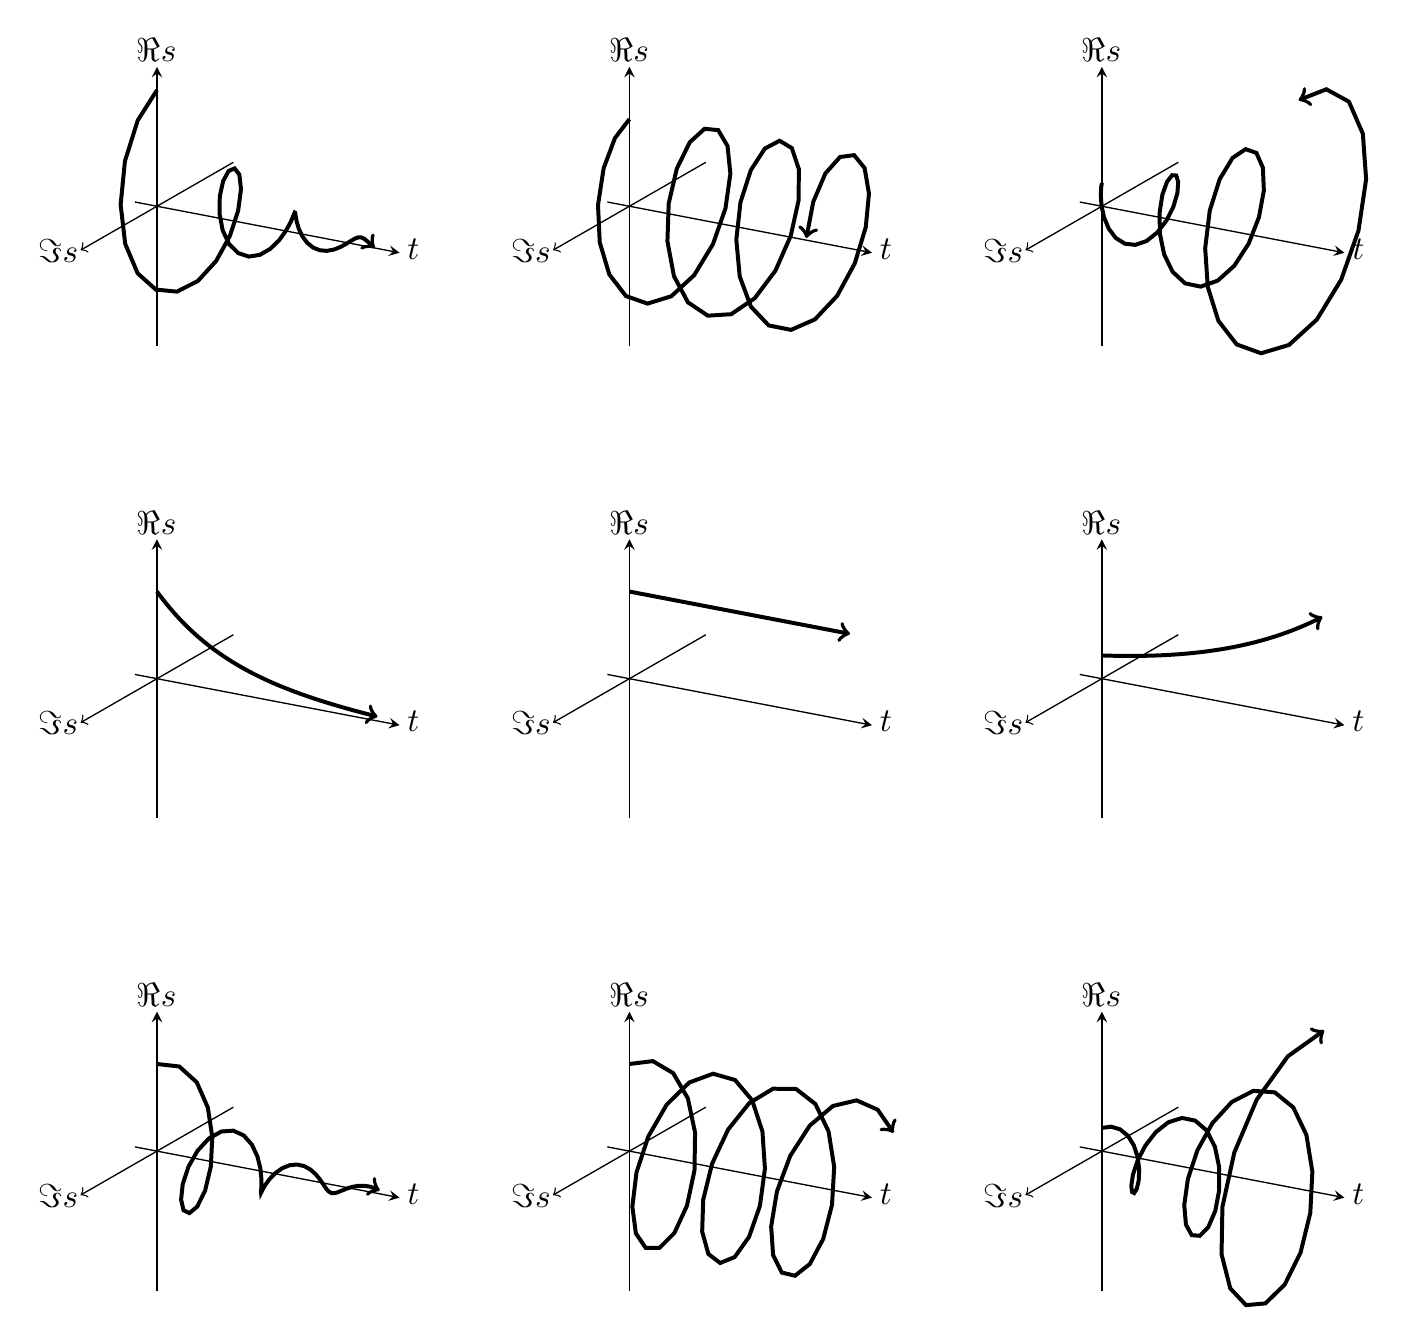
\begin{tikzpicture}[scale=1.2]
    \newcommand{\smp}{50}
    \newcommand{\gridA}{5}
    \newcommand{\gridB}{10}
    \newcommand{\fact}{0.75}
    \foreach \x in {0, \gridA, \gridB} {
        \foreach \y in {0, \gridA, \gridB} {
            \begin{axis}[
                    at={(\x cm, \y cm)},
                    anchor=south west,
                    width=6cm, height=6cm,
                    axis lines=middle, axis on top,
                    xlabel={$t$}, xmax=11, xmin=-1,
                    ylabel={$\Im s$}, ymax=1.2, ymin=-1.2,
                    zlabel={$\Re s$}, zmax=1.2, zmin=-1.2,
                    xtick=\empty, ytick=\empty, ztick=\empty,
                    y axis line style={<-},
                    enlargelimits=false,
                    x label style={at={(axis description cs:0.85,0.5)},anchor=north},
                    y label style={at={(axis description cs:0,0.5)},anchor=north},
                    z label style={at={(axis description cs:0.235,0.98)},anchor=north},
                    view={30}{20},
                ]

                \ifnum \x=0 \ifnum \y=0 % Bottom-Left
                \addplot3[domain=0:10, samples=\smp, samples y=0, very thick, ->]
                ({x}, {\fact*exp(-0.3*x)*sin(deg(2*x))}, {\fact*exp(-0.3*x)*cos(deg(2*x))});
                \fi \fi

                \ifnum \x=\gridA \ifnum \y=0 % Bottom-Center
                \addplot3[domain=0:10, samples=\smp, samples y=0, very thick, ->]
                ({x}, {\fact*sin(deg(2*x))}, {\fact*cos(deg(2*x))});
                \fi \fi

                \ifnum \x=\gridB \ifnum \y=0 % Bottom-Right
                \addplot3[domain=0:9.5, samples=\smp, samples y=0, very thick, ->]
                ({x}, {0.2*exp(0.2*x)*sin(deg(2*x))}, {0.2*exp(0.2*x)*cos(deg(2*x))});
                \fi \fi

                \ifnum \x=0 \ifnum \y=\gridA % Center-Left
                \addplot3[domain=0:10, samples=\smp, samples y=0, very thick, ->]
                ({x}, {0}, {\fact*exp(-0.3*x)});
                \fi \fi

                \ifnum \x=\gridA \ifnum \y=\gridA % Center
                \addplot3[domain=0:10, samples=\smp, samples y=0, very thick, ->]
                ({x}, {0}, {0.75});
                \fi \fi

                \ifnum \x=\gridB \ifnum \y=\gridA % Center-Right
                \addplot3[domain=0:10, samples=\smp, samples y=0, very thick, ->]
                ({x}, {0}, {0.2*exp(0.15*x)});
                \fi \fi

                \ifnum \x=0 \ifnum \y=\gridB % Top-Left
                \addplot3[domain=0:10, samples=\smp, samples y=0, very thick, ->]
                ({x}, {exp(-0.3*x)*sin(deg(-2*x))}, {exp(-0.3*x)*cos(deg(-2*x))});
                \fi \fi

                \ifnum \x=\gridA \ifnum \y=\gridB
                % Top-Center: Pure oscillation
                \addplot3[domain=0:10, samples=\smp, samples y=0, very thick, ->]
                ({x}, {\fact*sin(deg(-2*x))}, {0.75*cos(deg(-2*x))});
                \fi \fi

                \ifnum \x=\gridB \ifnum \y=\gridB
                % Top-Right: Growing spiral
                \addplot3[domain=0:9.5, samples=\smp, samples y=0, very thick, ->]
                ({x}, {0.2*exp(0.2*x)*sin(deg(-2*x))}, {0.2*exp(0.2*x)*cos(deg(-2*x))});
                \fi \fi
            \end{axis}
            }
        }
    \end{tikzpicture}
\end{document}
